\section{Method}\label{sec:method}
In this section, we first describe the describe the probabilistic framework that underlies the CMC algorithm, before introducing CMC in pseudocode (Algorithm \ref{alg:cmc}). We also detail the workflow we have found useful in applying this approach to analyse cell snapshot data and suggest practical remedies to issues we have encountered in using CMC (Figure \ref{fig:workflow}). A glossary of all the variables used in this paper is included as Table \ref{tab:variable_glossary}.

Experimental methods such as flow cytometry can measure single cell characteristics at a given point in time. Cells are typically destroyed by the measurement process and so rather than providing time series for each individual cell, the data consists of cross-sections or ``snapshots'' of sampled individuals from the population (Figure \ref{fig:time_series_v_snapshots}).

\begin{figure}[H]
	\centerline{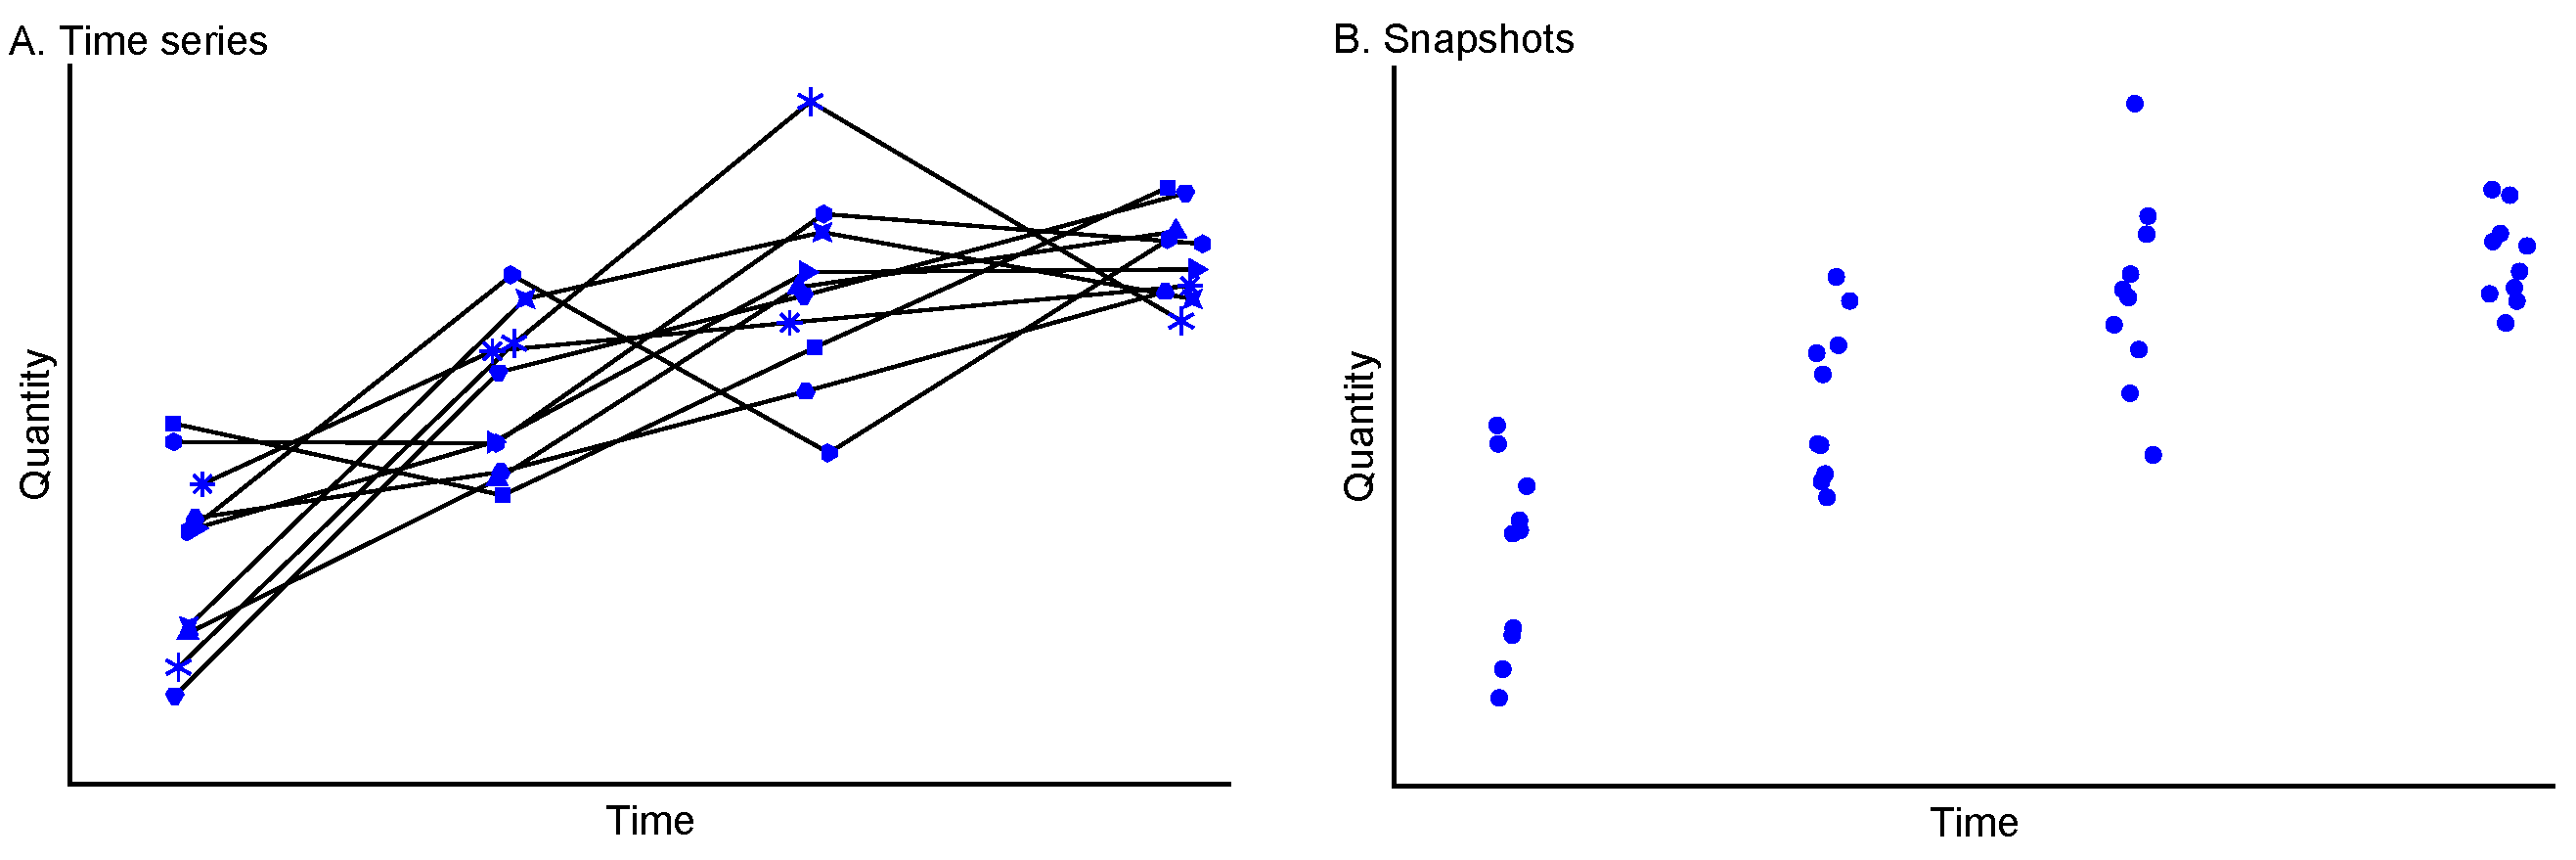
\includegraphics[width=\textwidth]{../figures/time_series_v_snapshots.pdf}}
	\caption{\textbf{Time series data (A) versus snapshot data (B) typical of single cell experiments.} In A that the cell identities are retained at each measurement point (indicated by given plot markers) whereas in the snapshot data in B, either this information is lost or, more often, cells are destroyed by the measurement process and so each observation corresponds to a distinct cell.}
	\label{fig:time_series_v_snapshots}
\end{figure}

We model the processes of an individual cell using a system of ordinary differential equations (ODEs), %where each element of the system describes the governing dynamics of a particular quantity of interest (for example, protein levels, RNA concentrations and so on),
%
\begin{equation}\label{eq:ode}
\begin{aligned}
\frac{d\boldsymbol{x}}{dt} &= \boldsymbol{f}(\boldsymbol{x}(t); \, \boldsymbol{\theta}), \quad \boldsymbol{f}: \R^k \times \R^p \mapsto \R^k, \\
\boldsymbol{x}(0) &= \boldsymbol{x}_0
\end{aligned}
\end{equation}
%
Note that in most circumstances, the initial state of the system, $\boldsymbol{x}(0)$, is unknown and it is convenient to include these as elements of $\boldsymbol{\theta}$ to be estimated. %The solution of eq. (\ref{eq:ODE}) is given by $\boldsymbol{x}(t) = g(t; \boldsymbol{\theta})$, where $\boldsymbol{x}(t)\in\mathbb{R}^k$ is a vector of outputs at time $t$ and $g(.)$ is a function that typically won't be analytically-determined; instead approximated via a numerical integration scheme.

In this paper, we assume variation characterised by snapshot data arises due to between-cell heterogeneity in the underlying parameters $\boldsymbol{\theta}$. Therefore, the evolution of the underlying state of cell $i$ is described by an idiosyncratic ODE,
%
\begin{equation} \label{eq:ode_i}
\begin{aligned}
\frac{d\boldsymbol{x}^{\{i\}}}{dt} &= \boldsymbol{f} \left( \boldsymbol{x}^{\{i\}}(t); \, \boldsymbol{\theta}^{\{i\}} \right),
                                      \quad \boldsymbol{f}: \R^k \times \R^p \mapsto \R^k, \\
\boldsymbol{x}^{\{i\}}(0) &= \boldsymbol{x}_0
\end{aligned}
\end{equation}
where $^{\{i\}}$ indicates the $i$th sample.
%
%with solution $\boldsymbol{x}^i(t) = g(t; \boldsymbol{\theta}^i)$.
The traditional (non-hierarchical) state-space approach to modelling dynamic systems supposes that measurement randomness generates output variation (Figure \ref{fig:data_generation}A). Our approach, by contrast, relies on the assumption that stochasticity in outputs is solely the result of variability in parameter values between cells (Figure \ref{fig:data_generation}B). Whether the assumption of ``perfect'' measurements is reasonable depends on the experimental details of  the system under investigation but we argue that our method nevertheless provides a useful approximation in many cases where the signal to noise ratio is high.

\begin{figure}[H]
	\centerline{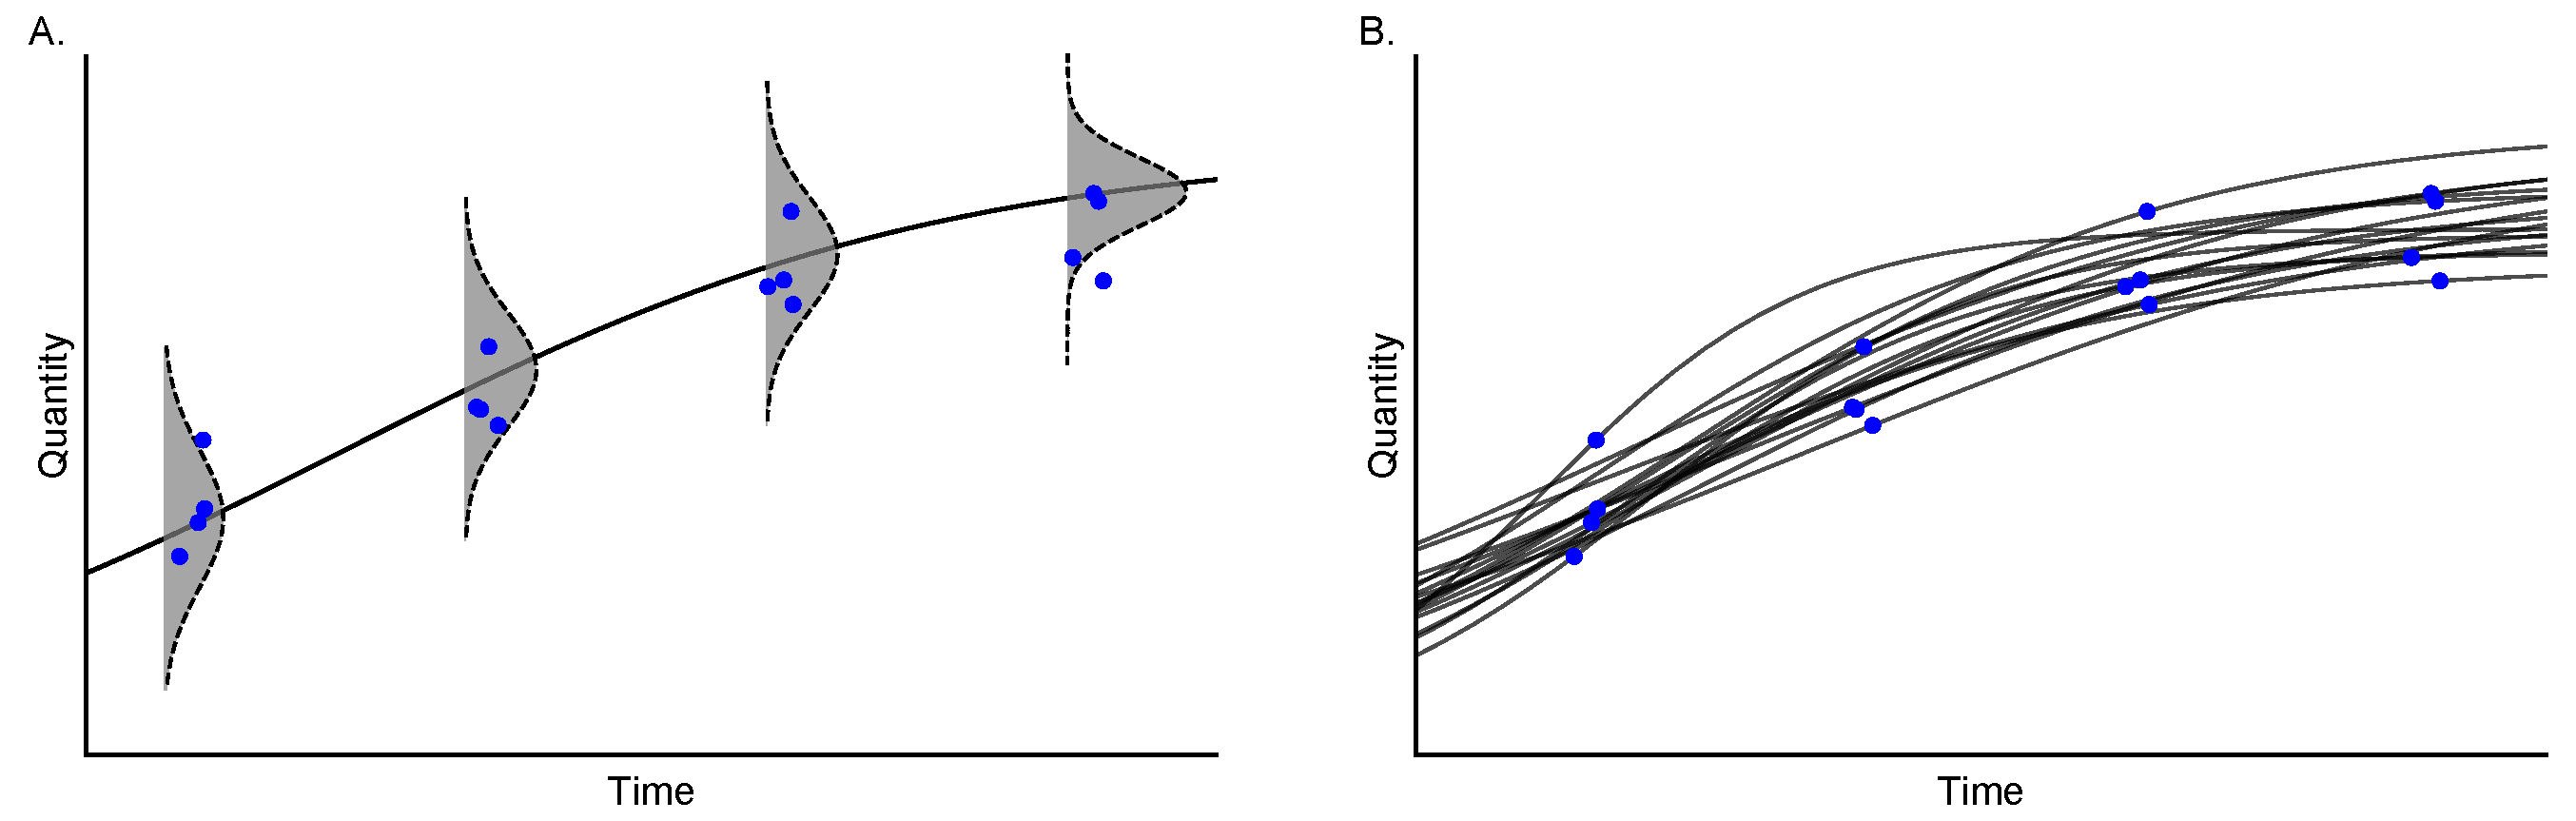
\includegraphics[width=\textwidth]{../figures/data_generation.pdf}}
	\caption{\textbf{Two ways to generate randomness in measured outputs: the state-space model (A) versus the parameter heterogeneity model (B).} For non-hierarchical state-space models (A), there is assumed to be a single ``true'' latent state where observations result from a noisy measurement process (grey histograms). For models with parameter heterogeneity (B), the uncertainty is generated by differences in cellular processes (black lines) between cells. Note that in both cases, individual cells are measured only once in their lifetime.}
	\label{fig:data_generation}
\end{figure}

\subsection{Emulation of experimental data}

We consider the situation in which we measure $m$ quantities of interest $q_j, j=1, \dots, m$.

We wish to emulate the experimental situation in which a set of observations is made. We simulate these experimental observations by solving the system of odes \eqref{eq:ode} multiple times for a range of values of parameters and calculate a (scalar-valued) quantity of interest for each value of the parameters.  Let $p(\boldsymbol{\theta})$ be a probability distribution characterising heterogeneity in cellular processes and consider the situation where we have $n_j$ observations of each quantity of interest $q_j$. These quantities of interest may be different functionals of the solution at the same time or the same functional at different times or a mixture of both. Define the vector containing a set of $m$ observations as
\begin{equation}
\boldsymbol{q}^\top = \left( q_1, q_2, \dots, q_m \right)
\end{equation}

\begin{algorithm}[H]
	\footnotesize
	\texttt{\\}
	\begin{algorithmic}
		\For{ $j=1$ to $m$ }
           \For{ $k=1$ to $n_j$ }
               \State $i=\sum_{l=1}^{j-1} n_l + k$
               \State Select $\boldsymbol{\theta}^{\{i\}} \sim p(\boldsymbol{\theta})$ and solve \eqref{eq:ode} for $x^{\{i\}}(t)$.
               \State Compute $q_j\left( x^{\{i\}}(t_j); \ \theta^{\{i\}} \right) \in \R$
            \EndFor
        \EndFor
	\end{algorithmic}
	\caption{Pseudocode for the generating raw snapshot data}\label{alg:raw}
\end{algorithm}
We define
\begin{equation}
\boldsymbol{y}(t_j)^\top = \left( q_j(\tilde x^{\{1\}}(t_j)), q_j(\tilde x^{\{2\}}(t_j)), \dots, q_j(\tilde x^{\{n_j}\}(t_j))  \right)^\top  \in \R^{n_j}
\end{equation}
and
\begin{equation}
  \boldsymbol{X}^\top = \left( \boldsymbol{y}(t_1), \boldsymbol{y}(t_2), \dots, \boldsymbol{y}(t_m) \right)^\top \in \R^s,
                        \quad \hbox{where} \; s = \sum_{j=1}^m n_j.
\end{equation}
The vector $\boldsymbol{X}$ defines the set of experimental observations, aka, raw snapshot data.

Raw snapshot data thus consists of measurements of individual cells with exact inference requiring simulating the underlying ODE system for each individual cell for each quantity of interest. This is cumbersome and impractical for the numbers of cells sampled in typical experimental setups and so, instead, we follow previous work and represent snapshot data using probability distributions \cite{hasenauer2011identification,hasenauer2014ode,loos2018hierarchical,dixit2018maximum}.
%The snapshots themselves can either be distributions of a single species or multiple species, which can be approximated by univariate and multivariate probability distributions respectively.
These probability distributions are characterised by parameter estimates $\hat{\Phi}$ for the output vector $\boldsymbol{Q}$ as determined by the output observations $\boldsymbol{X}$.
%The dimensionality of these probability distributions depends on the set of $m$ distinct observables $\tilde{\boldsymbol{x}}(\tilde{\boldsymbol{t}})=(x_{j_1}(t_1), x_{j_2}(t_2), ..., x_{j_m}(t_m))$ recorded by experimental measurements. Note that, $\tilde{\boldsymbol{x}}(\tilde{\boldsymbol{t}})$ corresponds to a particular set of measurements from a hypothetical cell and is distinct from $\boldsymbol{X}(\boldsymbol{t})$, which represents the full set of experimental outputs. The vector $\tilde{\boldsymbol{x}}(\tilde{\boldsymbol{t}})$ is hypothetical because in reality each cell is measured at a single timepoint (although we suppose measurements of different cellular attributes are possible contemporaneously).

\begin{table}[htbp]
\centering
\scriptsize
\begin{adjustwidth}{-0.5in}{-0.5in}%
\begin{tabularx}{1.1\textwidth}{lll}
Variable	                                                & Definition                                              & Dimension \\
\toprule
$\boldsymbol{x}(t)$                                     	& solution of ode                                         & $\R^k$ \\
$\boldsymbol{\theta}$                                     	& parameters                                              & $\R^p$ \\
$\boldsymbol{f}(\boldsymbol{x}(t); \, \boldsymbol{\theta})$	& RHS function of ode                                     & $\R^k$ \\
$\boldsymbol{x}^{\{i\}}(t)$                                 & solution of ode for cell $i$                            & $\R^k$ \\
&&\\
$q_j= q_j(\boldsymbol{x}(t_j))$                             & quantity of interest (qoi) $j$                          & $\R^1$ \\
$\boldsymbol{q}= \left( q_1, \dots, q_m \right)$            & all $m$ qoi                                             & $\R^m$ \\
&&\\
$q_j^{\{i\}}= q_j(\boldsymbol{x}^{\{i\}}(t_j))$             & quantity of interest $j$ for cell $i$                   & $\R^1$ \\
$\boldsymbol{y}_j=\left( q_j^{\{1\}}, \dots q_j^{\{n_j\}} \right)$  & qoi $j$ of cells $1, \dots, n_j$                & $\R^{n_j}$ \\
$\boldsymbol{X}=(\boldsymbol{y}_1,...,\boldsymbol{y}_m)$               & system observables (all qoi)                 & $\R^s, s=\sum_{j=1}^m n_j$ \\
&&\\
&&\\
$\Phi$ & parameters characterising output target distribution $p(\boldsymbol{q}|\Phi)$                                & $\R^m$ \\
$\Xi$  & parameters characterising parameter prior distribution $p(\boldsymbol{\theta}|\Xi)$                          & $\R^p$ \\
$\Psi$ & parameters characterising output prior distribution $p(\boldsymbol{q}|\Psi)$                                 & $\R^p$ \\
&&\\
$\hat{a}$ & estimates of any quantity $a$                                                                             & - \\
&&\\
$\Omega(\tilde{\boldsymbol{z}})$      & region of parameter space mapping to $\boldsymbol{q}=\boldsymbol{z}$          & $\R^p$ \\
$\mathcal{V}(\tilde{\boldsymbol{z}})$ & volume of parameter space mapping to $\boldsymbol{q}=\boldsymbol{z}$          & $\R^+$ \\
$V$                                   & total volume of parameter space                                               & $\R^+$ \\
\end{tabularx}
\caption{\textbf{Glossary of variable names used in this paper.}} %The dimensions of $\Phi$, $\Psi$ and $\Xi$ are listed as ``-'' since they depend on the form of the density used to represent the process and can be anywhere from $\mathbb{R}^1$ to $\mathbb{R}^\infty$. The variables are listed in the approximate order in which they appear in the text.}
\label{tab:variable_glossary}
\end{adjustwidth}
\end{table}


The goal of our inference process is to  characterise the probability distribution $p(\boldsymbol{\theta}|\boldsymbol{X})$ representing heterogeneity in cellular processes. The first step in our inference workflow is to fit the output distributions using probability distributions (Figure \ref{fig:workflow}(i)). We assume that the volume of observational data means the estimated probability distributions are approximate sufficient statistics of the outputs, meaning $p(\boldsymbol{\theta}|\hat{\Phi}) \approx p(\boldsymbol{\theta}|\boldsymbol{X})$.

\begin{figure}[H]
	\centerline{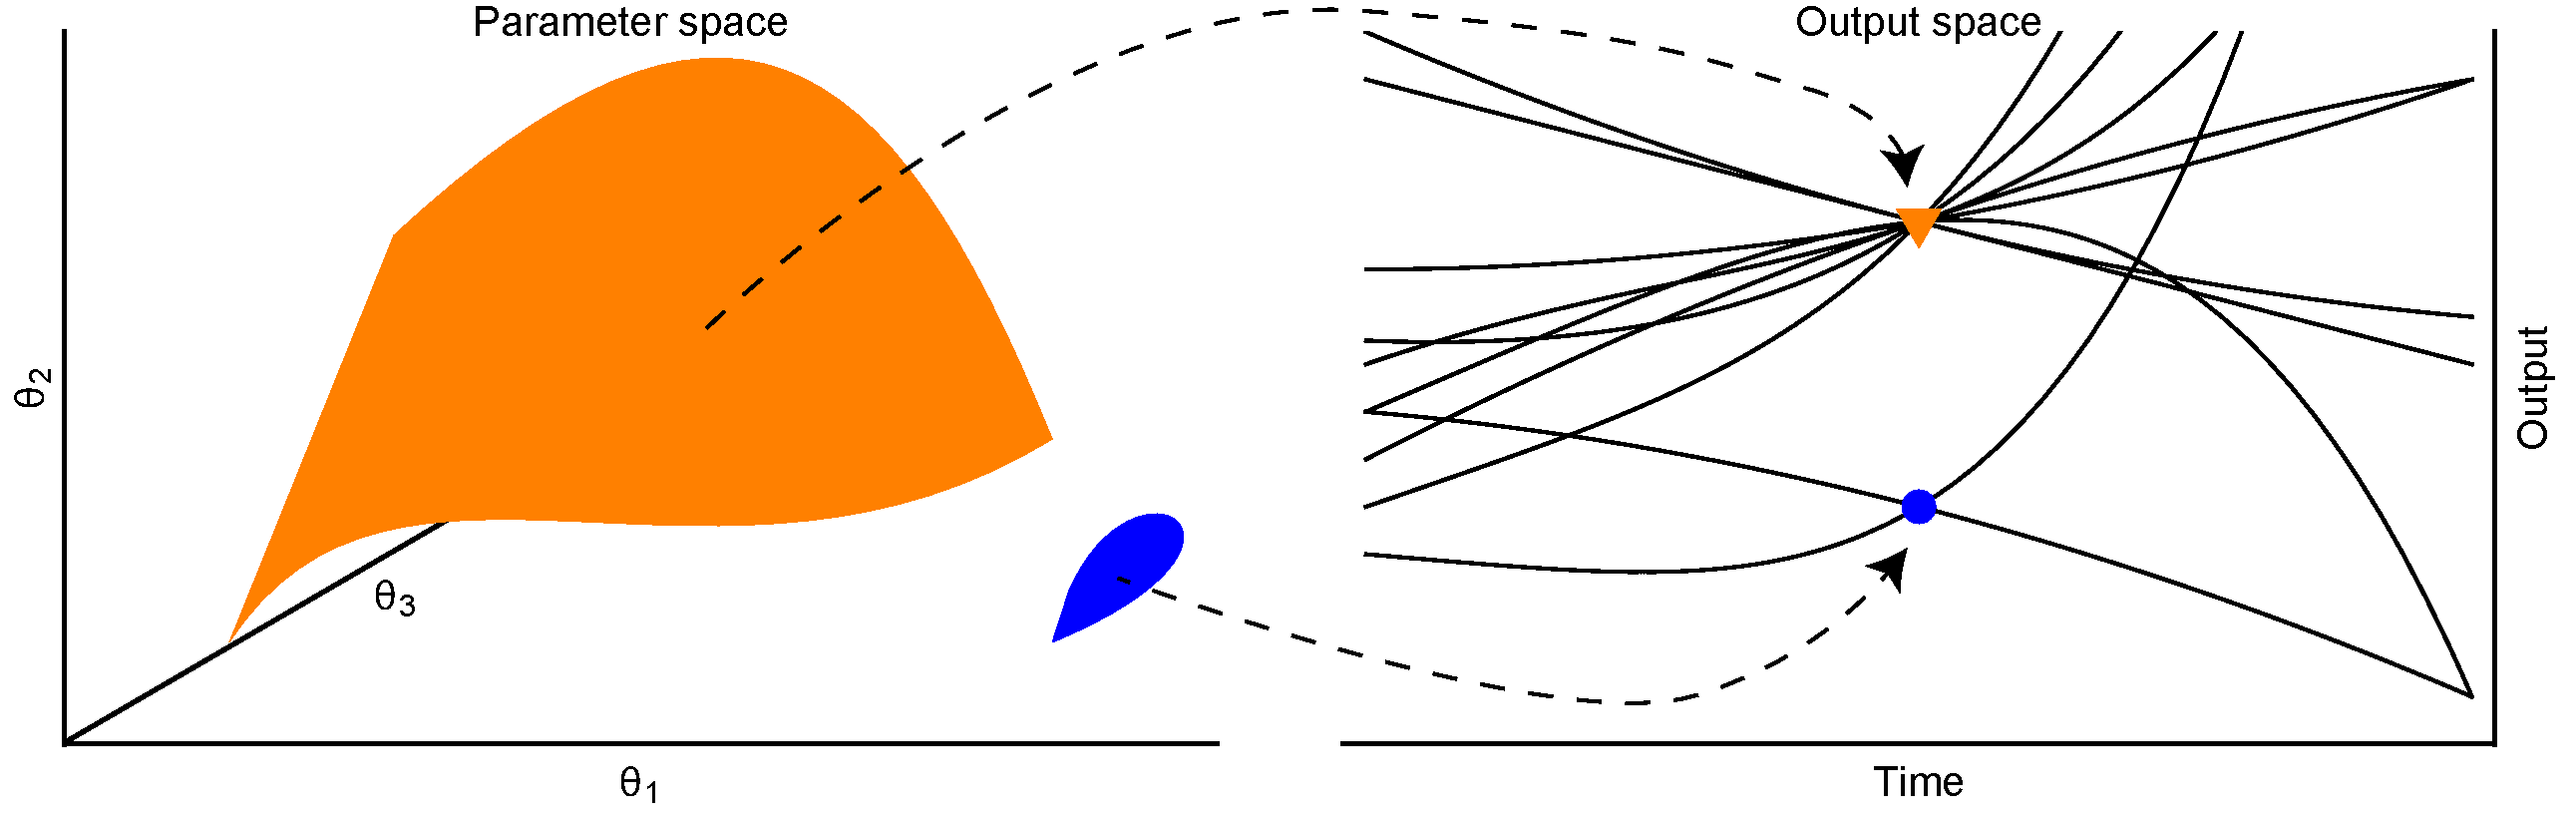
\includegraphics[width=\textwidth]{../figures/contour_volumes.pdf}}
	\caption{\textbf{The non-linear mapping from parameter values (left panel) to outputs (black lines; right panel) means different sized regions of parameter space (orange and blue surfaces; left panel) correspond to distinct output values (orange triangle and blue square; right panel).} In the right panel, each black line represents a distinct model simulation $g(t; \theta_1, \theta_2, \theta_3)$ and the triangle and square indicate outputs at a given point in time.}
	\label{fig:contour_volumes}
\end{figure}

\subsection{Inference}

We consider the underdetermined case where $m<p$,
The models we seek to fit to snapshot data mostly cannot be identified from the observations. This is often because the number of model parameters exceeds the dimensionality of the output distribution (that is, $m>k$) meaning there typically exist non-singular sets of parameter values mapping to a single set of output values. That is, each vector of observed outputs $\tilde{\boldsymbol{x}}\in\mathbb{R}^m$, can often be caused by many combinations of parameters although, due to the non-linearity of the map from parameters to outputs, the ``volume'' of these regions of parameter space, $\mathcal{V}(\tilde{\boldsymbol{x}})$, is a function of output (Figure \ref{fig:contour_volumes}). In what follows, we make clear the distinction between observables $\tilde{\boldsymbol{x}}(\tilde{\boldsymbol{t}})$ and the vector-valued function representing modelled outputs $\boldsymbol{g}(\tilde{\boldsymbol{t}}; \boldsymbol{\theta})=(g_{j_1}(t_1; \boldsymbol{\theta}),g_{j_2}(t_2; \boldsymbol{\theta}),...,g_{j_m}(t_m; \boldsymbol{\theta}))\in\mathbb{R}^m$ since the latter is a function whereas that latter is a numeric value; we also drop the $\tilde{\boldsymbol{t}}$ notation from following expressions to minimise clutter.

A consequence of this non-linear parameter to output geometry is that any target output distribution $p(\tilde{\boldsymbol{x}}|\hat{\Phi})$ does not correspond to a unique parameter distribution. For example, suppose $g(\theta_1, \theta_2) = \theta_1 + \theta_2$: the target distribution $\tilde{\boldsymbol{x}}\sim \mathcal{N}(0, 1)$ can be generated by any member of the set of parameter distributions $\sqrt{\eta} \theta_1 + \sqrt{1 - \eta} \theta_2$, where $\eta\in [0, 1]$ and $\theta_1, \theta_2 \sim \mathcal{N}(0, 1)$. This means that in order to ensure uniqueness of the ``posterior'' parameter distributions, we are required to specify ``prior'' distributions for the parameters, as in more traditional Bayesian inference. An additional consequence of the degeneracy of the mapping from parameters to outputs is that any sampling algorithm aimed at exploring posterior parameter space must account for the differential volumes of iso-output contours. Whilst we refer the interested reader to our companion paper on this subject [citation for tutorial paper published in Open Science], we provide a quick derivation of the posterior parameter distribution which accounts for the non-linear mapping.

To derive the posterior distribution of parameter values $p(\boldsymbol{\theta}|\hat{\Phi})$, we consider the joint density of parameters and outputs $p(\boldsymbol{\theta},(\boldsymbol{q}|\hat{\Phi}))$. This can be decomposed in two ways,
%
\begin{equation}\label{eq:joint}
  p( \boldsymbol{\theta}, (\boldsymbol{q}|\hat{\Phi}) )
= p( \boldsymbol{\theta}|(\boldsymbol{q}, \hat{\Phi}) ) \times p(\boldsymbol{q}|\hat{\Phi})
= p( \boldsymbol{q}|(\boldsymbol{\theta}, \hat{\Phi}) ) \times p(\boldsymbol{\theta}|\hat{\Phi}).
\end{equation}
%
Rearranging to obtain the posterior parameter distribution,
%
\begin{equation}
p(\boldsymbol{\theta}|\hat{\Phi})
= \frac{p(\boldsymbol{\theta}|\boldsymbol{q}, \hat{\Phi}) \times p(\boldsymbol{q}|\hat{\Phi})}{p(\boldsymbol{q}| \boldsymbol{\theta}, \hat{\Phi})}.
\end{equation}
%
Given parameters $\boldsymbol{\theta}$, the mapping from parameters to outputs is deterministic meaning
$p(\boldsymbol{q}| \boldsymbol{\theta}, \hat{\Phi})=\delta(\boldsymbol{q}(\boldsymbol{\theta}),\boldsymbol{\theta})$ is the Dirac delta function centred at $\boldsymbol{q}=\boldsymbol{q}(\boldsymbol{\theta})$.


In what follows, we assume that the conditional distribution $p(\boldsymbol{\theta}|\boldsymbol{q}, \hat{\Phi})$ is independent of the data, meaning it represents a conditional ``prior'', which can be manipulated by Bayes' rule,
%
\begin{equation}\label{eq:prior}
p(\boldsymbol{\theta}|\boldsymbol{q}(\boldsymbol{\theta})) = \frac{p(\boldsymbol{\theta})}{p(\boldsymbol{q}(\boldsymbol{\theta}))},
\end{equation}
%
where we have used the Dirac delta function for $p(\boldsymbol{q}|\boldsymbol{\theta})$. This results in the form of the posterior parameter distribution targeted by our sampling algorithm,
%
\begin{equation}\label{eq:posterior_input}
p(\boldsymbol{\theta}|\hat{\Phi}) = \frac{p(\boldsymbol{\theta})}{p(\boldsymbol{q}(\boldsymbol{\theta}))} p(\boldsymbol{q}(\boldsymbol{\theta})|\hat{\Phi}).
\end{equation}
%
Again, we refer to our companion piece [citation] for detailed explanation of eqs. (\ref{eq:prior}) \& (\ref{eq:posterior_input}) and instead here provide brief interpretation when considering a uniform prior on parameter space. In this case, $p(\boldsymbol{\theta}) = \frac{1}{V}$, where $V$ is the total volume of parameter space. The denominator term of eq. (\ref{eq:prior}) is the prior induced on output space by the prior over parameter space. For a uniform prior on parameter values, this is %just proportion of parameter space where $\boldsymbol{g}(\boldsymbol{\theta}) = \tilde{\boldsymbol{x}}$, meaning,
%
\begin{equation}\label{eq:contour_volume}
p(\boldsymbol{\theta}|\boldsymbol{q}(\boldsymbol{\theta})) = \frac{1}{\mathcal{V}(\boldsymbol{q}(\boldsymbol{\theta}))},
\end{equation}
%
where $\mathcal{V}(\boldsymbol{q}(\boldsymbol{\theta}))$ is the volume of parameter space occupied by the iso-output region $\Omega(\tilde{\boldsymbol{q}}) = \{\boldsymbol{\theta}: \boldsymbol{q}(\boldsymbol{\theta}) = \tilde{\boldsymbol{q}}\}$. Therefore a uniform prior over parameter space implies a prior structure where all  parameter values resulting in the same output $\tilde{\boldsymbol{q}}$ are given equal weighting.

\subsection{Implementation}

\subsubsection{Estimation of contour volumes}

The denominator term of eq. (\ref{eq:prior}) cannot be calculated apart from for some toy examples, meaning that exact sampling from the posterior parameter distribution of eq. (\ref{eq:posterior_input}) is not, in general, possible. We propose instead a computationally efficient sampling method to estimate $p(\boldsymbol{q}(\boldsymbol{\theta}))$, which forms the first step of our so-called ``Contour Monte Carlo'' (CMC) algorithm (Algorithm \ref{alg:cmc}; Figure \ref{fig:workflow}(ii)), where we estimate the volume of iso-output contours with output value $\boldsymbol{q}(\boldsymbol{\theta})$. This step involves repeated independent sampling from the prior distribution of parameters $\boldsymbol{\theta}^i\sim p(\boldsymbol{\theta}|\Xi)$, where, for completeness, we have conditioned on $\Xi$ parameterising our probability density. Each parameter sample is then converted into an output value $\tilde{\boldsymbol{x}}^i=\boldsymbol{g}(\boldsymbol{\theta}^i)$. The collection of output samples is then fitted using a vine copula kernel density estimator (KDE) \cite{nagler2016evading}, $(\tilde{\boldsymbol{x}}^1,\tilde{\boldsymbol{x}}^2,...,\tilde{\boldsymbol{x}}^{N_1})\sim p(\tilde{\boldsymbol{x}}|\hat{\Psi})$. Throughout the course of development of CMC, we have tested many forms of KDE and have found vine copula KDE is best suited to approximating the higher dimensional probability distributions required in practice.


\subsubsection{MCMC sampling}

The second step in our algorithm then uses Markov chain Monte Carlo (MCMC) to sample from an approximate version of eq. (\ref{eq:posterior_input}) with the estimated density $p(\boldsymbol{g}(\boldsymbol{\theta})|\hat{\Psi})$ replacing its corresponding estimand (Algorithm \ref{alg:cmc}; Figure \ref{fig:workflow}(iii)),
%
\begin{equation}\label{eq:posterior_input_estimated}
p(\boldsymbol{\theta}|\hat{\Phi},\Xi,\hat{\Psi}) = \frac{p(\boldsymbol{\theta}|\Xi)}{p(\boldsymbol{g}(\boldsymbol{\theta})|\hat{\Psi})} p(\boldsymbol{g}(\boldsymbol{\theta})|\hat{\Phi}).
\end{equation}
%

\begin{algorithm}[H]
	\footnotesize
	\texttt{\\}
	\begin{algorithmic}
		\Procedure{CMC}{$\boldsymbol{X}(\boldsymbol{t}), \Xi, N_1, N_2$}\Comment{Sample from posterior parameter distribution}
		\State $\hat{\Phi} = \Call{SnapshotEstimator}{\boldsymbol{X}(\boldsymbol{t})}$
		\State $\hat{\Psi} = \Call{ContourVolumeEstimator}{\Xi}$
		\State $(\boldsymbol{\theta}_1,...,\boldsymbol{\theta}_{N_2}) = \Call{MCMC}{\hat{\Phi},\Xi, \hat{\Psi},N_2}$
		\State $\text{converged} = \Call{CompareOutputToTarget}{(\boldsymbol{\theta}_1,...,\boldsymbol{\theta}_{N_2}), \hat{\Psi}}$
		\If{converged$\neq$1}
		\State $(\boldsymbol{\theta}_1,...,\boldsymbol{\theta}_{N_2})$=\Call{ContourVolumeEstimator}{$\hat{\Phi}, \Xi, N_1', N_2'$}
		\State where, $N_1' > N_1$ and/or $N_2' > N_2$ \Comment{Rerun contour volume estimation and/or MCMC with larger sample sizes}
		\EndIf
		\State \Return $(\boldsymbol{\theta}_1,...,\boldsymbol{\theta}_{N_2})$
		\EndProcedure
	\end{algorithmic}

	\texttt{\\}
	\begin{algorithmic}
		\Procedure{SnapshotEstimator}{$\boldsymbol{X}(\boldsymbol{t})$}\Comment{Fit density to snapshot observations}
		\State $\boldsymbol{X}(\boldsymbol{t}) \sim p(\tilde{\boldsymbol{x}}|\hat{\Phi})$
		\State \Return $\hat{\Phi}$
		\EndProcedure
	\end{algorithmic}
	
	\texttt{\\}
	\begin{algorithmic}
		\Procedure{ContourVolumeEstimator}{$\Xi, N_1$}\Comment{Estimate volume of contours}
		\For{$i$ in $1:N_1$}
		\State $\boldsymbol{\theta}_i\sim p(\boldsymbol{\theta}|\Xi)$ \Comment{Sample from prior density}
		\State $\tilde{\boldsymbol{x}}_i = \boldsymbol{g}(\boldsymbol{\theta}_i)$ \Comment{Calculate corresponding output value}
		\EndFor
		\State $(\tilde{\boldsymbol{x}}_1,\tilde{\boldsymbol{x}}_2,...,\tilde{\boldsymbol{x}}_{N_1}) \sim p(\tilde{\boldsymbol{x}}|\hat{\Psi})$ \Comment{Fit vine copula kernel density estimator to output values.}
		\State \Return $\hat{\Psi}$
		\EndProcedure
	\end{algorithmic}

	\texttt{\\}
	\begin{algorithmic}
		\Procedure{MCMC}{$\hat{\Phi},\Xi, \hat{\Psi}, N_2$}\Comment{Random Walk Metropolis algorithm targeting posterior parameter distribution.}
		\State $\boldsymbol{\theta}_0 \sim \pi(.)$ \Comment{Sample from arbitrary initialisation distribution}
		\For{$i$ in $1:N_2$}
		\State $\boldsymbol{\theta}_i'\sim \mathcal{N}(\boldsymbol{\theta}_{i-1},\boldsymbol{\Sigma})$ \Comment{Propose new parameter values for parameters}
		\State $r = \left[p(\boldsymbol{\theta}'|\Xi) p(\boldsymbol{g}(\boldsymbol{\theta})|\hat{\Psi})p(\boldsymbol{g}(\boldsymbol{\theta}')|\hat{\Phi})\right] / \left[p(\boldsymbol{\theta}|\Xi) p(\boldsymbol{g}(\boldsymbol{\theta}')|\hat{\Psi})p(\boldsymbol{g}(\boldsymbol{\theta})|\hat{\Phi})\right]$\Comment{Metropolis acceptance ratio.}
		\State $u\sim U(0,1)$ \Comment{Sample from uniform distribution}
		\If{$r > u$}
		\State $\boldsymbol{\theta}_i = \boldsymbol{\theta}_i'$ \Comment{Accept proposal}
		\Else
		\State $\boldsymbol{\theta}_i = \boldsymbol{\theta}_{i-1}$ \Comment{Reject proposal}
		\EndIf
		\EndFor
		\State \Return $(\boldsymbol{\theta}_1,...,\boldsymbol{\theta}_{N_2})$
		\EndProcedure
	\end{algorithmic}

	\texttt{\\}
	\begin{algorithmic}
			\Procedure{CompareOutputToTarget}{$(\boldsymbol{\theta}_1,...,\boldsymbol{\theta}_{N_2}), \hat{\Phi}$}\Comment{Check output distribution close to target}
		\For{$i$ in $1:N_2$}
		\State $\tilde{\boldsymbol{x}}_i = \boldsymbol{g}(\boldsymbol{\theta}_i)$ \Comment{Compute output for each parameter sample}
		\EndFor
		\If{$(\tilde{\boldsymbol{x}}_1,\tilde{\boldsymbol{x}}_2,...,\tilde{\boldsymbol{x}}_{N_2})\sim p(\tilde{\boldsymbol{x}}|\hat{\Phi})?$} \Comment{Compare outputs with target}
		\State \Return 1 \Comment{If outputs sufficiently close then converged}
		\Else
		\State \Return 0
		\EndIf
		\EndProcedure
	\end{algorithmic}

	\caption{Pseudocode for the Contour Monte Carlo algorithm for sampling from the posterior parameter distribution of eq. (\ref{eq:posterior_input_estimated}). Here we provide code for the Random Walk Metropolis algorithm for the MCMC sampling but for the examples in \S \ref{sec:results}, we use an adaptive MCMC algorithm \cite{johnstone2016uncertainty}. A definition of all variables is provided in Table \ref{tab:variable_glossary}.}\label{alg:cmc}
\end{algorithm}

\begin{figure}[H]
	\centerline{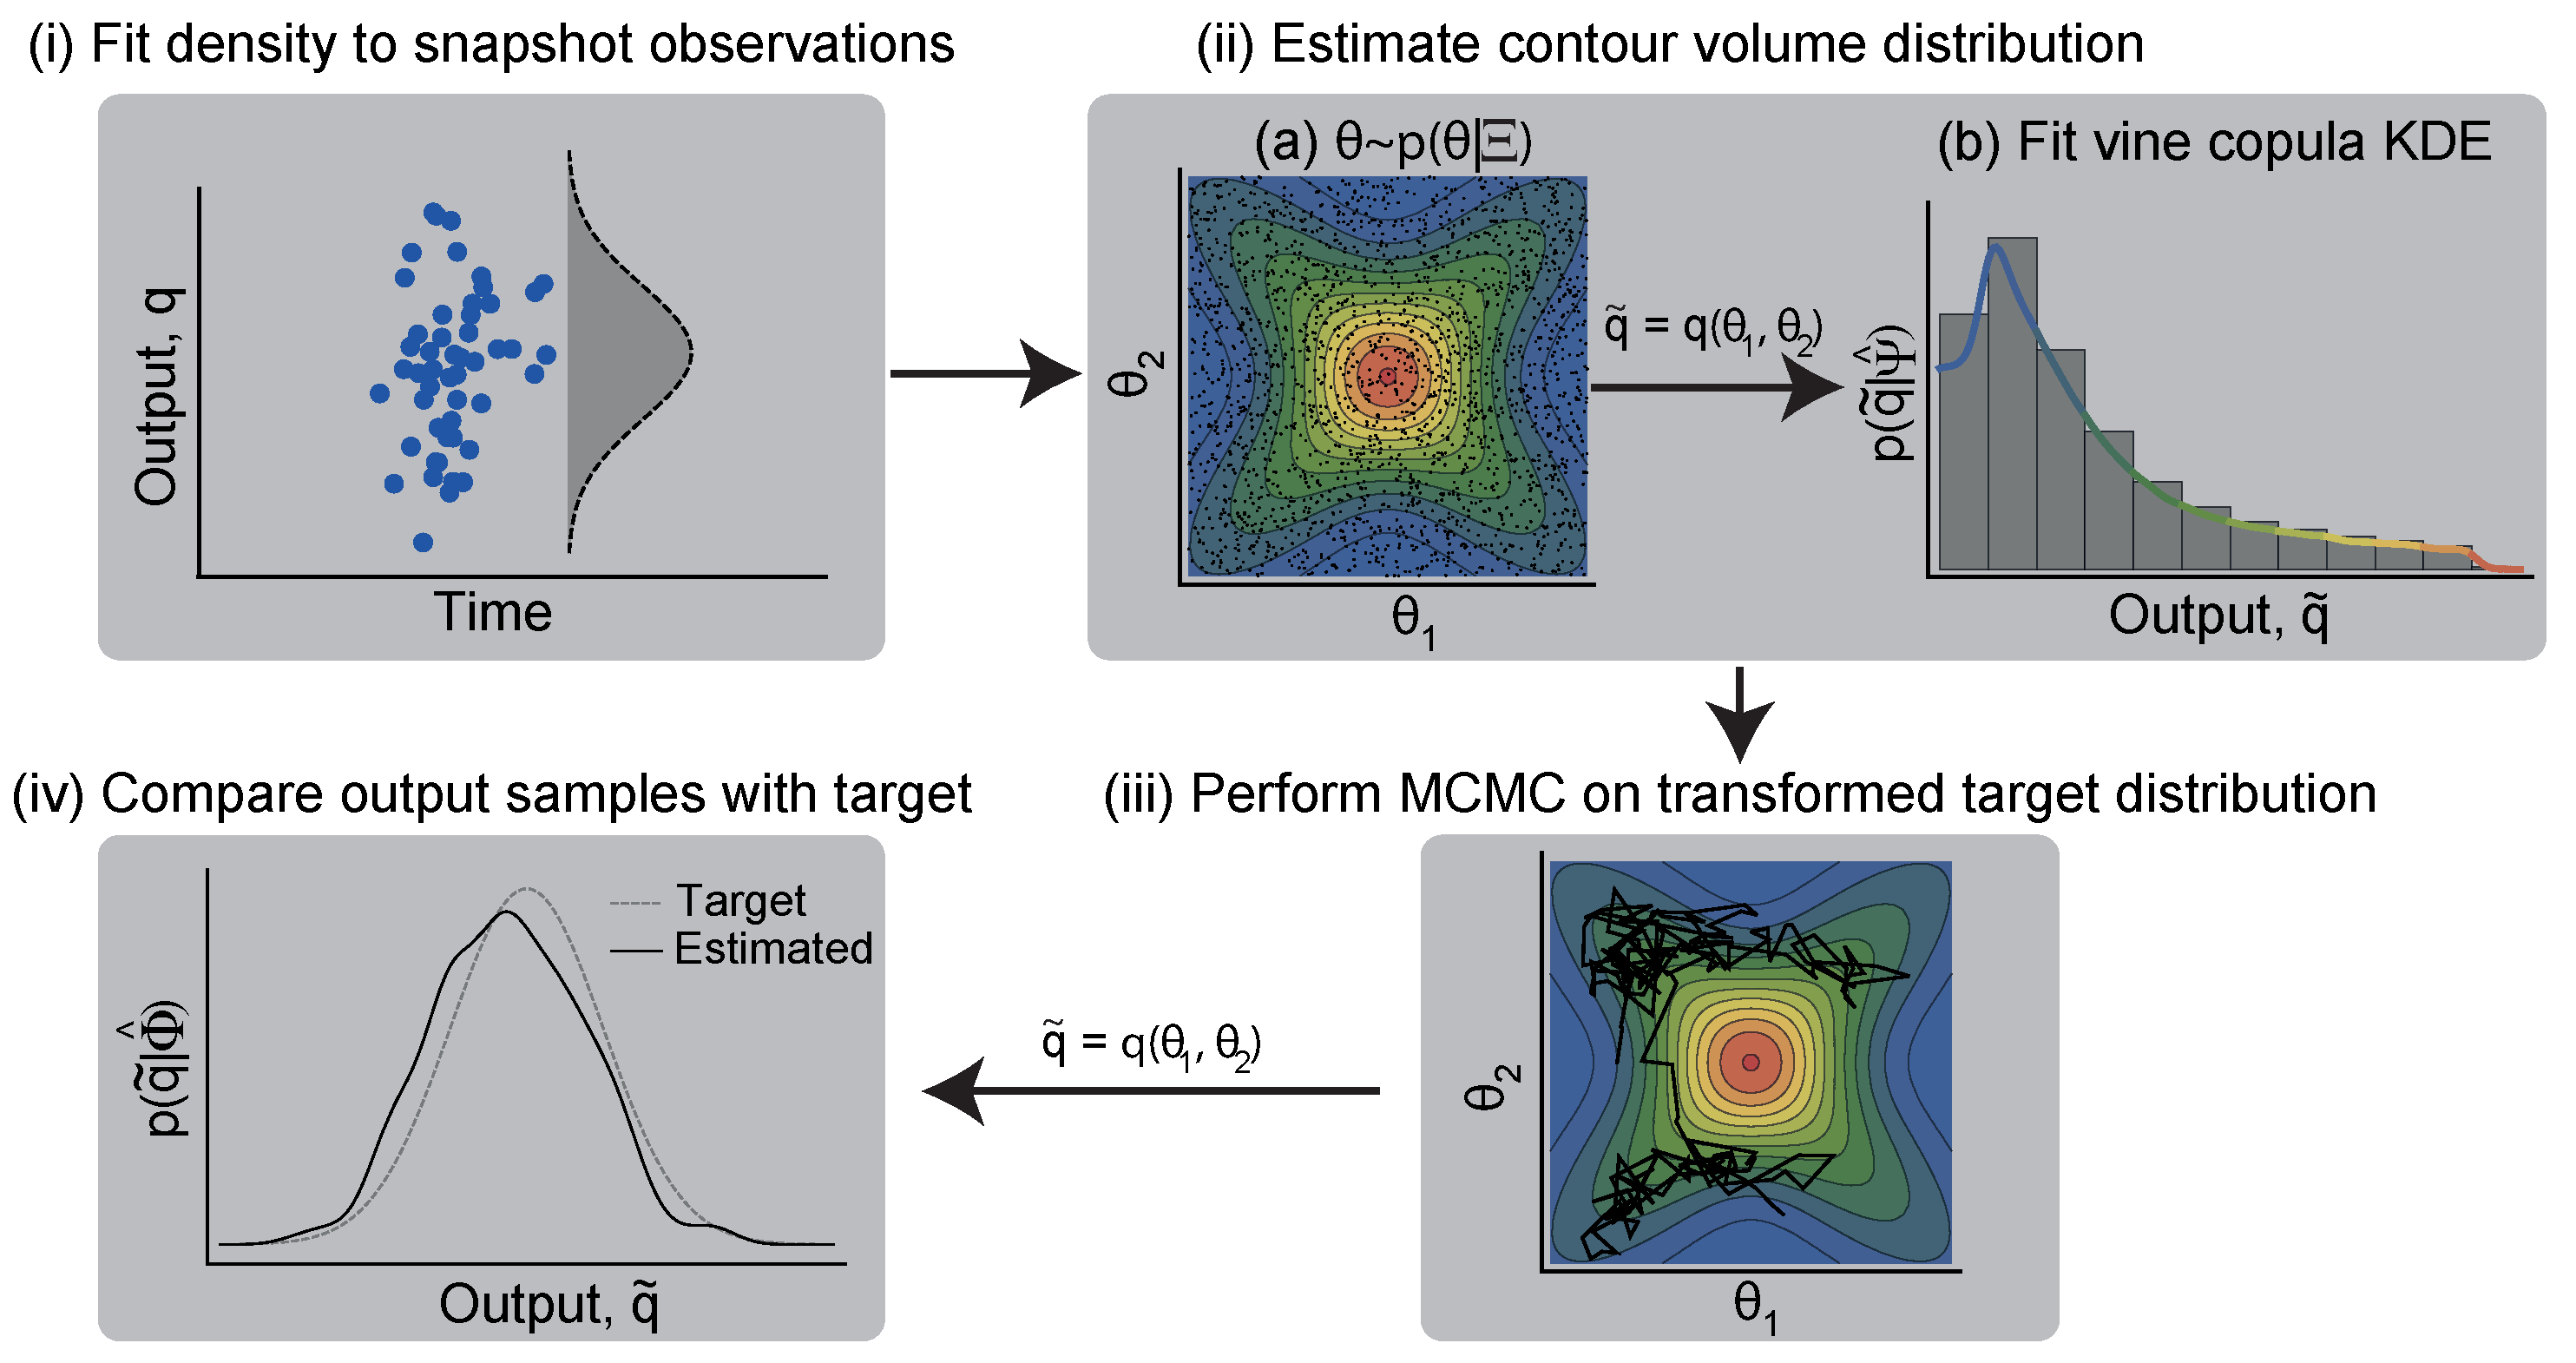
\includegraphics[width=\textwidth]{../figures/workflow.pdf}}
	\caption{\textbf{The workflow for using Contour Monte Carlo to estimate cell population heterogeneity.} In (iii), the distribution targeted is given by eq. (\ref{eq:posterior_input_estimated}). The variables used in this figure are defined in the text and Table \ref{tab:variable_glossary}.}
	\label{fig:workflow}
\end{figure}

\subsubsection{Reconstruction of target output distribution}

The final step in CMC is to transform parameter samples from the MCMC into outputs, then compare the sampled outputs with the target distribution (Figure \ref{fig:workflow}(iv)). Asymptotically (in terms of the sample size of both sampling steps), CMC produces a sample of parameter values $(\boldsymbol{\theta}^{\{1\}},\boldsymbol{\theta}^{\{2\}},...)$ which, when transformed to outputs, corresponds to the target distribution $p(\boldsymbol{q}|\hat{\Psi})$. In developing CMC, we have found that a finite sample of modest size for both steps of CMC results in parameter samples that, when transformed, often represent reasonable approximations of the target. There are however occasions when this is not the case and we have found this final confirmatory step indispensable since it frequently highlights inadequacies in the contour volume estimation or the MCMC, meaning more samples from either or both of these steps are required. It may also be necessary to tweak hyperparameters of the KDE to ensure reasonable approximation in the contour volume estimation step. If the target distribution is sensitive to the contour volume estimates, this may also indicate that the target snapshot distribution is incompatible with the model: here, we make no claims on existence of a solution to the inverse problem, only that, if one should exist, Contour Monte Carlo is a pragmatic approach to approximate it by sampling. A useful way to diagnose whether the target distribution can be produced from the model and specified priors is to examine the output values from the contour volume estimation step of CMC. If the majority of probability mass of the target lies outside the bounds of the bulk simulated output values obtained by independent sampling from the prior, then the model and/or chosen prior is unlikely to be invertible to this particular target.

In generating our results in \S\ref{sec:results}, for the contour volume estimation step, we assumed sample sizes were sufficient if the output samples from the MCMC provided a reasonable approximation to the target, although we recognise that future work should refine this process further. For the MCMC step, we use adaptive covariance MCMC (see SOM of \cite{johnstone2016uncertainty}) to sample from the target distribution, as we have found that it provides a considerable speed-up over Random Walk Metropolis \cite{metropolis1953equation,lambert2018Student}. We also use the Gelman-Rubin convergence statistic $\hat{R}$ which provides a heuristic measurement of convergence \cite{lambert2018Student,gelman1992inference}, and use a threshold of $\hat{R}\leq\sim 1.1$ to diagnose convergence.
